\documentclass[letter,11pt]{article}

\usepackage[spanish,es-nodecimaldot]{babel}
\usepackage[utf8]{inputenc}

\usepackage{lmodern}
\usepackage[T1]{fontenc}
\usepackage{textcomp}

\usepackage{framed}
\usepackage[svgnames]{xcolor}
\colorlet{shadecolor}{Gainsboro!50}

\usepackage[shortlabels]{enumitem}
\usepackage{graphicx}
\usepackage{pstricks}
\usepackage{amsmath}

\usepackage{anysize}
\marginsize{3cm}{2cm}{2cm}{3cm}

\usepackage{fancyhdr}
\usepackage{lastpage}
\pagestyle{fancy}
\fancyhf{}
\fancyhead[LE,RO]{Física Básica II}
\fancyfoot[CO,CE]{\thepage\ de \pageref{LastPage}}

\special{papersize=215.9mm,279.4mm}

\usepackage[
    pdfauthor={Carlos Eduardo Caballero Burgoa},%
    pdftitle={Física Básica II},%
    pdfsubject={Tarea 19},%
    colorlinks,%
    citecolor=black,%
    filecolor=black,%
    linkcolor=black,%
    urlcolor=black,
    breaklinks]{hyperref}
\usepackage{breakurl}

\newcommand{\blankpage}{
\newpage
\thispagestyle{empty}
\mbox{}
\newpage
}

\renewcommand{\arraystretch}{1.2}

\begin{document}

\begin{center}
    {\Large \bf{Tarea \#19}}
\end{center}

Un anillo (aro) uniforme y delgado de $R = 0.5 [m]$ y masa $m = 0.4 [kg]$ esta
suspendido verticalmente por uno de sus extremos.

\begin{figure}[!h]
\centering
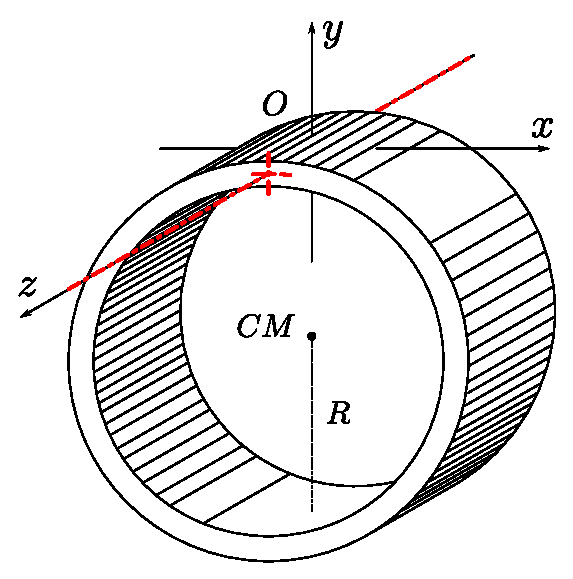
\includegraphics[scale=0.65]{resources/f1.eps}
\end{figure}

Si $\phi_0 = 10^\circ$ y $\Omega_0 = \dot{\psi}_0 = 0 [rad/s]$ para $t = 0 [s]$,
calcular:

\begin{enumerate}[a)]
    \item La frecuencia angular de oscilación, el periodo de oscilación y la
        frecuencia de oscilación.
    \item La ecuación $\psi = \psi(t)$.
    \item La ecuación $\Omega = \dot{\psi} = \dot{\psi}(t)$.
    \item La ecuación $\alpha = \ddot{\psi} = \ddot{\psi}(t)$.
    \item Las ecuaciones paramétricas del movimiento en $XY$.
\end{enumerate}


\vspace{0.5cm}
\textbf{Solución:} \\

\textbf{(a)} \\

Sabemos que el momento de inercia en el centro de masa de un cilindro hueco de
pared delgada es:

\begin{equation*}
    I_{CM} = M R^2
\end{equation*}

y con ayuda del teorema de los ejes paralelos:

\begin{equation*}
    I_{P} = I_{CM} + M d^2
\end{equation*}

Calculamos el momento de inercia sobre el eje de rotación en un extremo:

\begin{equation}
    I_{O} = M R^2 + M R^2 = 2 M R^2
\end{equation}

Sabiendo que:

\begin{equation*}
    \ddot{\psi} + \frac{m g d}{I_O} \psi = 0
\end{equation*}

y comparando con la ecuación de un oscilador armónico simple:

\begin{equation*}
    \ddot{x} + \omega^2 x = 0
\end{equation*}

Obtenemos la frecuencia angular de oscilación ($\omega$):

\begin{equation}
    \omega = \sqrt{ \frac{m\, g\, d}{I_O} } = \sqrt{ \frac{m g R}{2 m R^2} } = \sqrt{ \frac{g}{2 R} } = \sqrt{ \frac{9.8}{2(0.5)} } = 3.1305 [rad/s]
\end{equation}

El periodo de oscilación ($T$):

\begin{equation}
    T = \frac{2 \pi}{\omega} = \frac{2 \pi}{3.1305} = 2.0071 [s]
\end{equation}

Y la frecuencia de oscilación ($\nu$):

\begin{equation}
    f = \frac{1}{T} = \frac{1}{2.0071} = 0.4982 [Hz]
\end{equation}

\textbf{(b)} \\

La solución general de un oscilador armónico simple es:

\begin{equation*}
    \psi = A \cdot cos(\omega t - \phi)
\end{equation*}

Considerando las condiciones iniciales para $t = 0$:

\begin{equation*}
    \psi_0 = 10^\circ \cdot \frac{\pi [rad]}{180^\circ} = \frac{\pi}{18} [rad]
\end{equation*}
\begin{equation*}
    \dot{\psi_0} = 0
\end{equation*}

Obtenemos las siguientes ecuaciones:

\begin{equation}
    \begin{cases}
        \frac{\pi}{18} = A \cdot cos(- \phi) \\
        0 = -A \cdot 3.1305 \cdot sen(- \phi)
    \end{cases}
\end{equation}

Despejando $\phi$ de la segunda ecuación:

\begin{equation*}
    0 = sen(-\phi)
\end{equation*}
\begin{equation*}
    0 = sen(\phi)
\end{equation*}
\begin{equation}
    \phi = arcsen(0) = 0
\end{equation}

Y se calcula $A$ de la primera ecuación:

\begin{equation}
    A = \frac{\pi}{18 \cdot cos(0)} = \frac{\pi}{18} = 0.1745 [rad]
\end{equation}

Por tanto:

\begin{equation*}
    \psi = A \cdot cos(\omega \cdot t - \phi)
\end{equation*}
\begin{equation}
    \psi = 0.1745 \cdot cos(3.1305 \cdot t)
\end{equation}

\textbf{(c)} \\

Derivando la función $\psi$:

\begin{equation*}
    \dot{\psi} = - A\, \omega \cdot sen(\omega \cdot t - \phi)
\end{equation*}
\begin{equation*}
    \dot{\psi} = - 0.1745 \cdot 3.1305 \cdot sen(3.1305 \cdot t)
\end{equation*}
\begin{equation}
    \Omega = \dot{\psi} = - 0.5464 \cdot sen(3.1305 \cdot t)
\end{equation}

\textbf{(d)} \\

Derivando la función $\dot{\psi}$:

\begin{equation*}
    \ddot{\psi} = - A\, \omega^2 \cdot cos(\omega \cdot t - \phi)
\end{equation*}
\begin{equation*}
    \ddot{\psi} = -0.1745 \cdot (3.1305)^2 \cdot cos(3.1305 \cdot t)
\end{equation*}
\begin{equation}
    \alpha = \ddot{\psi} = -1.7104 \cdot cos(3.1305 \cdot t)
\end{equation}

\textbf{(e)} \\

A partir de las relaciones trigonométricas, sabemos:

\begin{equation*}
    x(t) = R \cdot sen (\psi) = R \cdot sen (\psi) = R \cdot sen(A \cdot cos(\omega t))
\end{equation*}
\begin{equation}
    x(t) = 0.5 \cdot sen ( 0.1745 \cdot cos (3.1305\, t) ) [m]
\end{equation}

\begin{equation*}
    y(t) = -R \cdot cos (\psi) = - R \cdot cos(\psi) = - R \cdot cos(A \cdot cos(\omega t))
\end{equation*}
\begin{equation}
    y(t) = - 0.5 \cdot cos ( 0.1745 \cdot cos (3.1305\, t) ) [m]
\end{equation}

Por tanto:

\begin{equation}
    \vec{r}(t) = 0.5 \cdot sen(0.1745 \cdot cos(3.1305\, t))\, \hat{i} - 0.5 \cdot cos(0.1745 \cdot cos(3.1305\, t))\, \hat{j}
\end{equation}

Derivando las funciones de posición se hallan las ecuaciones de velocidad, con
la ayuda de la regla de la cadena:

\begin{equation*}
    \frac{d}{dt} \left[f(g(t))\right] = f'(g(t))\, g'(t)
\end{equation*}

\begin{equation*}
    x'(t) = R \cdot cos(A \cdot cos(\omega t))\, (A (-sen(\omega t)))\, \omega
\end{equation*}
\begin{equation*}
    x'(t) = -R\, A \omega \cdot cos(A \cdot cos(\omega t)) \cdot sen(\omega t)
\end{equation*}
\begin{equation}
    x'(t) = -0.2732 \cdot cos(0.1745 \cdot cos(3.1305\, t)) \cdot sen(3.1305\, t)
\end{equation}

\begin{equation*}
    y'(t) = -R \cdot (-sen(A \cdot cos(\omega t)))\, (A (-sen(\omega t)))\, \omega
\end{equation*}
\begin{equation*}
    y'(t) = -R\, A \omega \cdot sen(A \cdot cos(\omega t)) \cdot sen(\omega t)
\end{equation*}
\begin{equation}
    y'(t) = -0.2732 \cdot sen(0.1745 \cdot cos(3.1305\, t)) \cdot sen(3.1305\, t)
\end{equation}

Derivando las funciones de velocidad se hallan las ecuaciones de aceleración,
con la ayuda de la derivada de un producto:

\begin{equation*}
    \frac{d}{dt} \left[f(t) \cdot g(t)\right] = f'(t) \cdot g(t) + f(t) \cdot g'(t)
\end{equation*}

\begin{equation*}
    x''(t) = -R\, A \omega\, [ A \omega \cdot sen(A \cdot cos(\omega t)) \cdot sen^2(\omega t) + \omega \cdot cos(A \cdot cos(\omega t)) \cdot cos(\omega t)]
\end{equation*}
\begin{equation*}
    x''(t) = -R\, A \omega^2\, [ A \cdot sen(A \cdot cos(\omega t)) \cdot sen^2(\omega t) + cos(A \cdot cos(\omega t)) \cdot cos(\omega t)]
\end{equation*}
\begin{equation}
    \begin{split}
        x''(t) = -0.1493 \cdot sen(0.1745 \cdot cos(3.1305 t)) \cdot sen^2(3.1305 t) \\
                 -0.8552 \cdot cos(0.1745 \cdot cos(3.1305t)) \cdot cos(3.1305t)
    \end{split}
\end{equation}

\begin{equation*}
    y''(t) = -R\, A \omega\, [ -A \omega \cdot cos(A \cdot cos(\omega t)) \cdot sen^2(\omega t) + \omega \cdot sen(A \cdot cos(\omega t)) \cdot cos(\omega t)]
\end{equation*}
\begin{equation*}
    y''(t) = R\, A \omega^2\, [A \cdot cos(A \cdot cos(\omega t)) \cdot sen^2(\omega t) - sen(A \cdot cos(\omega t)) \cdot cos(\omega t)]
\end{equation*}
\begin{equation}
    \begin{split}
        y''(t) = 0.1493 \cdot cos(0.1745 \cdot cos(3.1305 t)) \cdot sen^2(3.1305 t) \\
                 -0.8552 \cdot sen(0.1745 \cdot cos(3.1305t)) \cdot cos(3.1305t)
    \end{split}
\end{equation}

\end{document}

